\documentclass{article}\usepackage[]{graphicx}\usepackage[]{color}
%% maxwidth is the original width if it is less than linewidth
%% otherwise use linewidth (to make sure the graphics do not exceed the margin)
\makeatletter
\def\maxwidth{ %
  \ifdim\Gin@nat@width>\linewidth
    \linewidth
  \else
    \Gin@nat@width
  \fi
}
\makeatother

\definecolor{fgcolor}{rgb}{0.345, 0.345, 0.345}
\newcommand{\hlnum}[1]{\textcolor[rgb]{0.686,0.059,0.569}{#1}}%
\newcommand{\hlstr}[1]{\textcolor[rgb]{0.192,0.494,0.8}{#1}}%
\newcommand{\hlcom}[1]{\textcolor[rgb]{0.678,0.584,0.686}{\textit{#1}}}%
\newcommand{\hlopt}[1]{\textcolor[rgb]{0,0,0}{#1}}%
\newcommand{\hlstd}[1]{\textcolor[rgb]{0.345,0.345,0.345}{#1}}%
\newcommand{\hlkwa}[1]{\textcolor[rgb]{0.161,0.373,0.58}{\textbf{#1}}}%
\newcommand{\hlkwb}[1]{\textcolor[rgb]{0.69,0.353,0.396}{#1}}%
\newcommand{\hlkwc}[1]{\textcolor[rgb]{0.333,0.667,0.333}{#1}}%
\newcommand{\hlkwd}[1]{\textcolor[rgb]{0.737,0.353,0.396}{\textbf{#1}}}%

\usepackage{framed}
\makeatletter
\newenvironment{kframe}{%
 \def\at@end@of@kframe{}%
 \ifinner\ifhmode%
  \def\at@end@of@kframe{\end{minipage}}%
  \begin{minipage}{\columnwidth}%
 \fi\fi%
 \def\FrameCommand##1{\hskip\@totalleftmargin \hskip-\fboxsep
 \colorbox{shadecolor}{##1}\hskip-\fboxsep
     % There is no \\@totalrightmargin, so:
     \hskip-\linewidth \hskip-\@totalleftmargin \hskip\columnwidth}%
 \MakeFramed {\advance\hsize-\width
   \@totalleftmargin\z@ \linewidth\hsize
   \@setminipage}}%
 {\par\unskip\endMakeFramed%
 \at@end@of@kframe}
\makeatother

\definecolor{shadecolor}{rgb}{.97, .97, .97}
\definecolor{messagecolor}{rgb}{0, 0, 0}
\definecolor{warningcolor}{rgb}{1, 0, 1}
\definecolor{errorcolor}{rgb}{1, 0, 0}
\newenvironment{knitrout}{}{} % an empty environment to be redefined in TeX

\usepackage{alltt}
\usepackage{alltt}
\usepackage{amsmath}
\usepackage[sc]{mathpazo}
\usepackage[T1]{fontenc}
\usepackage{geometry}
\geometry{verbose,tmargin=2.5cm,bmargin=2.5cm,lmargin=2.5cm,rmargin=2.5cm}
\setcounter{secnumdepth}{2}
\setcounter{tocdepth}{2}
\usepackage{url}
\usepackage[unicode=true,pdfusetitle,
 bookmarks=true,bookmarksnumbered=true,bookmarksopen=true,bookmarksopenlevel=2,
 breaklinks=false,pdfborder={0 0 1},backref=false,colorlinks=false]
 {hyperref}
\hypersetup{
 pdfstartview={XYZ null null 1}}
 
\title{Code for new Supplementary Figure - post SIM rejection} 
 
\usepackage{breakurl}
\IfFileExists{upquote.sty}{\usepackage{upquote}}{}
\begin{document}
\maketitle
%\SweaveOpts{concordance=TRUE}



\section{Get the combined datasets for all the scenarios}

Load the necessary libraries:
\begin{knitrout}
\definecolor{shadecolor}{rgb}{0.969, 0.969, 0.969}\color{fgcolor}\begin{kframe}
\begin{alltt}
\hlkwd{library}\hlstd{(ggplot2)}
\hlkwd{library}\hlstd{(clusterGeneration)}
\end{alltt}


{\ttfamily\noindent\itshape\color{messagecolor}{\#\# Loading required package: MASS}}\begin{alltt}
\hlkwd{source}\hlstd{(}\hlstr{"functions.R"}\hlstd{)}
\end{alltt}
\end{kframe}
\end{knitrout}

Load the files representing the summary for each scenario and save the results in a single dataframe, \textttt{VarsAll}:
\begin{knitrout}
\definecolor{shadecolor}{rgb}{0.969, 0.969, 0.969}\color{fgcolor}\begin{kframe}
\begin{alltt}
\hlstd{allFiles} \hlkwb{<-} \hlkwd{list.files}\hlstd{(}\hlstr{"simResultsComb"}\hlstd{)}

\hlcom{##save the three Vars for the different combinations}
\hlstd{VarsAll} \hlkwb{<-} \hlkwd{expand.grid}\hlstd{(}\hlkwc{p} \hlstd{=} \hlkwd{c}\hlstd{(}\hlnum{5}\hlstd{,}\hlnum{10}\hlstd{,}\hlnum{15}\hlstd{,}\hlnum{20}\hlstd{),}
                       \hlkwc{randVar} \hlstd{=} \hlnum{1}\hlopt{:}\hlnum{5}\hlstd{,}
                       \hlkwc{het} \hlstd{=} \hlkwd{c}\hlstd{(}\hlnum{0.2}\hlstd{,} \hlnum{1}\hlstd{,} \hlnum{5}\hlstd{),}
                       \hlkwc{sampleType} \hlstd{=} \hlkwd{c}\hlstd{(}\hlstr{"same"}\hlstd{,} \hlstr{"diff"}\hlstd{),}
                       \hlkwc{I} \hlstd{=} \hlkwd{c}\hlstd{(}\hlnum{10}\hlstd{,}\hlnum{20}\hlstd{))}

\hlstd{VarsAll}\hlopt{$}\hlstd{known} \hlkwb{<-} \hlstd{VarsAll}\hlopt{$}\hlstd{unknown} \hlkwb{<-} \hlstd{VarsAll}\hlopt{$}\hlstd{univKnown} \hlkwb{<-} \hlstd{VarsAll}\hlopt{$}\hlstd{univ} \hlkwb{<-}
  \hlstd{VarsAll}\hlopt{$}\hlstd{knownEmpWithin} \hlkwb{<-} \hlstd{VarsAll}\hlopt{$}\hlstd{univKnownEmpWithin} \hlkwb{<-} \hlnum{NA}

\hlkwa{for}\hlstd{(file} \hlkwa{in} \hlnum{1}\hlopt{:}\hlkwd{length}\hlstd{(allFiles))}
\hlstd{\{}
    \hlkwd{load}\hlstd{(}\hlkwd{paste}\hlstd{(}\hlstr{"simResultsComb"}\hlstd{, allFiles[file],} \hlkwc{sep}\hlstd{=}\hlstr{"/"}\hlstd{))}

    \hlstd{rowNr} \hlkwb{<-} \hlkwd{gsub}\hlstd{(}\hlstr{"combine_cost_of_estimation_post_SIM"}\hlstd{,} \hlstr{""}\hlstd{, allFiles[file])}
    \hlstd{rowNr} \hlkwb{<-} \hlkwd{gsub}\hlstd{(}\hlstr{".RData"}\hlstd{,} \hlstr{""}\hlstd{, rowNr)}
    \hlstd{rowNr} \hlkwb{<-} \hlkwd{as.numeric}\hlstd{(rowNr)}

    \hlstd{VarsAll[rowNr,} \hlkwd{c}\hlstd{(}\hlstr{"p"}\hlstd{,}\hlstr{"randVar"}\hlstd{,}\hlstr{"het"}\hlstd{,}\hlstr{"sampleType"}\hlstd{,}\hlstr{"I"}\hlstd{,}
                     \hlstr{"univ"}\hlstd{,}\hlstr{"univKnown"}\hlstd{,}
                     \hlstr{"unknown"}\hlstd{,}\hlstr{"known"}\hlstd{)]} \hlkwb{<-}
      \hlstd{Vars[rowNr,} \hlkwd{c}\hlstd{(}\hlstr{"p"}\hlstd{,}\hlstr{"randVar"}\hlstd{,}\hlstr{"het"}\hlstd{,}\hlstr{"sampleType"}\hlstd{,}\hlstr{"I"}\hlstd{,}
                    \hlstr{"univ"}\hlstd{,}\hlstr{"univKnown"}\hlstd{,}
                    \hlstr{"unknown"}\hlstd{,}\hlstr{"known"}\hlstd{)]}

    \hlcom{##get number of studies, number of parameters, scenario number, etc}
    \hlstd{p} \hlkwb{<-} \hlstd{VarsAll[rowNr,} \hlstr{"p"}\hlstd{]}
    \hlstd{randVar} \hlkwb{<-} \hlstd{VarsAll[rowNr,} \hlstr{"randVar"}\hlstd{]}
    \hlstd{het} \hlkwb{<-} \hlstd{VarsAll[rowNr,} \hlstr{"het"}\hlstd{]}
    \hlstd{sampleType} \hlkwb{<-} \hlstd{VarsAll[rowNr,} \hlstr{"sampleType"}\hlstd{]}
    \hlstd{I} \hlkwb{<-} \hlstd{VarsAll[rowNr,} \hlstr{"I"}\hlstd{]}

    \hlcom{##get theoretical variances of multivariate and univariate estimators}
    \hlstd{varMult} \hlkwb{<-} \hlstd{varUniv} \hlkwb{<-} \hlstd{varUnivT1} \hlkwb{<-} \hlstd{varUnivT2} \hlkwb{<-} \hlkwd{matrix}\hlstd{(}\hlnum{0}\hlstd{, p, p)}

    \hlcom{##simulate Sigma again}
    \hlcom{##set.seed(381048+1940*randVar)}
    \hlcom{##Sigma <- cov2cor(genPositiveDefMat(p)$Sigma)*het}

    \hlstd{D} \hlkwb{<-} \hlkwd{diag}\hlstd{(}\hlkwd{diag}\hlstd{(Sigma))}

    \hlkwa{for}\hlstd{(site} \hlkwa{in} \hlnum{1}\hlopt{:}\hlstd{I)}
    \hlstd{\{}
      \hlcom{##StudyEmpVars[[site]] <- StudyEmpVars[[site]] + Sigma}

      \hlstd{varMult} \hlkwb{<-} \hlstd{varMult}\hlopt{+}\hlkwd{solve}\hlstd{(StudyEmpVars[[site]]}\hlopt{+}\hlstd{Sigma)}

      \hlstd{Uisite} \hlkwb{<-} \hlkwd{diag}\hlstd{(}\hlkwd{diag}\hlstd{(StudyEmpVars[[site]]))}

      \hlstd{varUnivT1} \hlkwb{<-} \hlstd{varUnivT1}\hlopt{+}\hlkwd{solve}\hlstd{(Uisite}\hlopt{+}\hlstd{D)}
      \hlstd{varUnivT2} \hlkwb{<-} \hlstd{varUnivT2}\hlopt{+}
        \hlkwd{solve}\hlstd{(Uisite}\hlopt{+}\hlstd{D)} \hlopt \hlstd{(StudyEmpVars[[site]]}\hlopt{+}\hlstd{Sigma)} \hlopt \hlkwd{solve}\hlstd{(Uisite}\hlopt{+}\hlstd{D)}
    \hlstd{\}}

    \hlstd{varMult} \hlkwb{<-} \hlkwd{solve}\hlstd{(varMult)}
    \hlstd{varUnivT1} \hlkwb{<-} \hlkwd{solve}\hlstd{(varUnivT1)}
    \hlstd{varUniv} \hlkwb{<-} \hlstd{varUnivT1} \hlopt \hlstd{varUnivT2} \hlopt \hlstd{varUnivT1}

    \hlstd{VarsAll[rowNr,} \hlkwd{c}\hlstd{(}\hlstr{"knownEmpWithin"}\hlstd{,}\hlstr{"univKnownEmpWithin"}\hlstd{)]} \hlkwb{<-}
      \hlkwd{c}\hlstd{(varMult[}\hlnum{1}\hlstd{], varUniv[}\hlnum{1}\hlstd{])}
\hlstd{\}}
\hlstd{VarsAll}\hlopt{$}\hlstd{Ratio} \hlkwb{<-} \hlstd{VarsAll}\hlopt{$}\hlstd{known}\hlopt{/}\hlstd{VarsAll}\hlopt{$}\hlstd{unknown}
\hlstd{VarsAll}\hlopt{$}\hlstd{RelEff} \hlkwb{<-} \hlstd{VarsAll}\hlopt{$}\hlstd{unknown}\hlopt{/}\hlstd{VarsAll}\hlopt{$}\hlstd{univ}
\hlstd{VarsAll}\hlopt{$}\hlstd{RelEffT} \hlkwb{<-} \hlstd{VarsAll}\hlopt{$}\hlstd{known}\hlopt{/}\hlstd{VarsAll}\hlopt{$}\hlstd{univKnown}
\hlstd{VarsAll}\hlopt{$}\hlstd{RelEffTAsympt} \hlkwb{<-} \hlstd{VarsAll}\hlopt{$}\hlstd{knownEmpWithin}\hlopt{/}\hlstd{VarsAll}\hlopt{$}\hlstd{univKnownEmpWithin}

\hlkwd{range}\hlstd{(VarsAll}\hlopt{$}\hlstd{Ratio)}
\end{alltt}
\begin{verbatim}
## [1] 0.8521896 0.9982430
\end{verbatim}
\end{kframe}
\end{knitrout}

\begin{knitrout}
\definecolor{shadecolor}{rgb}{0.969, 0.969, 0.969}\color{fgcolor}\begin{kframe}
\begin{alltt}
\hlcom{##add a column that specifically gives the value of Sigma^2 (from het)}
\hlstd{VarsAll}\hlopt{$}\hlstd{Sigma2} \hlkwb{<-} \hlstr{""}
\hlstd{VarsAll}\hlopt{$}\hlstd{Sigma2[VarsAll}\hlopt{$}\hlstd{het} \hlopt{==} \hlnum{0.2}\hlstd{]} \hlkwb{<-} \hlstr{"Sigma^2 = 1/5"}
\hlstd{VarsAll}\hlopt{$}\hlstd{Sigma2[VarsAll}\hlopt{$}\hlstd{het} \hlopt{==} \hlnum{1}\hlstd{]} \hlkwb{<-} \hlstr{"Sigma^2 = 1"}
\hlstd{VarsAll}\hlopt{$}\hlstd{Sigma2[VarsAll}\hlopt{$}\hlstd{het} \hlopt{==} \hlnum{5}\hlstd{]} \hlkwb{<-} \hlstr{"Sigma^2 = 5"}
\hlstd{VarsAll}\hlopt{$}\hlstd{Sigma2} \hlkwb{<-} \hlkwd{factor}\hlstd{(VarsAll}\hlopt{$}\hlstd{Sigma2,}
                         \hlkwc{levels}\hlstd{=} \hlkwd{c}\hlstd{(}\hlstr{"Sigma^2 = 1/5"}\hlstd{,} \hlstr{"Sigma^2 = 1"}\hlstd{,} \hlstr{"Sigma^2 = 5"}\hlstd{))}

\hlstd{VarsAllSame} \hlkwb{<-} \hlstd{VarsAll[VarsAll}\hlopt{$}\hlstd{sampleType}\hlopt{==}\hlstr{"same"}\hlstd{,]}
\hlstd{VarsAllDiff} \hlkwb{<-} \hlstd{VarsAll[VarsAll}\hlopt{$}\hlstd{sampleType}\hlopt{==}\hlstr{"diff"}\hlstd{,]}

\hlcom{##get the minimum value for Sigma^2 = 5}
\hlkwd{min}\hlstd{(VarsAll}\hlopt{$}\hlstd{RelEff[VarsAll}\hlopt{$}\hlstd{Sigma2} \hlopt{==} \hlstr{"Sigma^2 = 5"}\hlstd{])}
\end{alltt}
\begin{verbatim}
## [1] 0.9404613
\end{verbatim}
\begin{alltt}
\hlcom{##change format so it's ggplot-friendly}
\hlstd{RelEffSame} \hlkwb{<-}
  \hlkwd{rbind}\hlstd{(}\hlkwd{cbind}\hlstd{(}\hlkwd{as.matrix}\hlstd{(VarsAllSame[,}\hlkwd{c}\hlstd{(}\hlstr{"p"}\hlstd{,} \hlstr{"I"}\hlstd{,} \hlstr{"randVar"}\hlstd{,} \hlstr{"RelEff"}\hlstd{),]),}\hlstr{"RelEff"}\hlstd{),}
        \hlkwd{cbind}\hlstd{(}\hlkwd{as.matrix}\hlstd{(VarsAllSame[,}\hlkwd{c}\hlstd{(}\hlstr{"p"}\hlstd{,} \hlstr{"I"}\hlstd{,} \hlstr{"randVar"}\hlstd{,} \hlstr{"RelEffT"}\hlstd{),]),}\hlstr{"RelEffT"}\hlstd{),}
        \hlkwd{cbind}\hlstd{(}\hlkwd{as.matrix}\hlstd{(VarsAllSame[,}\hlkwd{c}\hlstd{(}\hlstr{"p"}\hlstd{,} \hlstr{"I"}\hlstd{,} \hlstr{"randVar"}\hlstd{,} \hlstr{"RelEffTAsympt"}\hlstd{),]),}\hlstr{"RelEffTAsympt"}\hlstd{))}
\hlkwd{colnames}\hlstd{(RelEffSame)[}\hlnum{5}\hlstd{]} \hlkwb{<-} \hlstr{"Estimate"}
\hlstd{RelEffSame} \hlkwb{<-} \hlkwd{as.data.frame}\hlstd{(RelEffSame)}
\hlstd{RelEffSame}\hlopt{$}\hlstd{Sigma2} \hlkwb{<-} \hlkwd{factor}\hlstd{(}\hlkwd{c}\hlstd{(}\hlkwd{as.character}\hlstd{(VarsAllSame}\hlopt{$}\hlstd{Sigma2),} \hlkwd{as.character}\hlstd{(VarsAllSame}\hlopt{$}\hlstd{Sigma2),}
                              \hlkwd{as.character}\hlstd{(VarsAllSame}\hlopt{$}\hlstd{Sigma2)),}
                            \hlkwc{levels} \hlstd{=} \hlkwd{c}\hlstd{(}\hlstr{"Sigma^2 = 1/5"}\hlstd{,} \hlstr{"Sigma^2 = 1"}\hlstd{,} \hlstr{"Sigma^2 = 5"}\hlstd{))}

\hlstd{RelEffSame}\hlopt{$}\hlstd{p} \hlkwb{<-} \hlkwd{as.numeric}\hlstd{(}\hlkwd{as.character}\hlstd{(RelEffSame}\hlopt{$}\hlstd{p))}
\hlstd{RelEffSame}\hlopt{$}\hlstd{RelEff} \hlkwb{<-} \hlkwd{as.numeric}\hlstd{(}\hlkwd{as.character}\hlstd{(RelEffSame}\hlopt{$}\hlstd{RelEff))}

\hlcom{##}

\hlstd{RelEffDiff} \hlkwb{<-}
  \hlkwd{rbind}\hlstd{(}\hlkwd{cbind}\hlstd{(}\hlkwd{as.matrix}\hlstd{(VarsAllDiff[,}\hlkwd{c}\hlstd{(}\hlstr{"p"}\hlstd{,} \hlstr{"I"}\hlstd{,} \hlstr{"randVar"}\hlstd{,} \hlstr{"RelEff"}\hlstd{),]),}\hlstr{"RelEff"}\hlstd{),}
        \hlkwd{cbind}\hlstd{(}\hlkwd{as.matrix}\hlstd{(VarsAllDiff[,}\hlkwd{c}\hlstd{(}\hlstr{"p"}\hlstd{,} \hlstr{"I"}\hlstd{,} \hlstr{"randVar"}\hlstd{,} \hlstr{"RelEffT"}\hlstd{),]),}\hlstr{"RelEffT"}\hlstd{),}
        \hlkwd{cbind}\hlstd{(}\hlkwd{as.matrix}\hlstd{(VarsAllDiff[,}\hlkwd{c}\hlstd{(}\hlstr{"p"}\hlstd{,} \hlstr{"I"}\hlstd{,} \hlstr{"randVar"}\hlstd{,} \hlstr{"RelEffTAsympt"}\hlstd{),]),}\hlstr{"RelEffTAsympt"}\hlstd{))}
\hlkwd{colnames}\hlstd{(RelEffDiff)[}\hlnum{5}\hlstd{]} \hlkwb{<-} \hlstr{"Estimate"}
\hlstd{RelEffDiff} \hlkwb{<-} \hlkwd{as.data.frame}\hlstd{(RelEffDiff)}
\hlstd{RelEffDiff}\hlopt{$}\hlstd{Sigma2} \hlkwb{<-} \hlkwd{factor}\hlstd{(}\hlkwd{c}\hlstd{(}\hlkwd{as.character}\hlstd{(VarsAllDiff}\hlopt{$}\hlstd{Sigma2),} \hlkwd{as.character}\hlstd{(VarsAllDiff}\hlopt{$}\hlstd{Sigma2),}
                              \hlkwd{as.character}\hlstd{(VarsAllDiff}\hlopt{$}\hlstd{Sigma2)),}
                            \hlkwc{levels} \hlstd{=} \hlkwd{c}\hlstd{(}\hlstr{"Sigma^2 = 1/5"}\hlstd{,} \hlstr{"Sigma^2 = 1"}\hlstd{,} \hlstr{"Sigma^2 = 5"}\hlstd{))}

\hlstd{RelEffDiff}\hlopt{$}\hlstd{p} \hlkwb{<-} \hlkwd{as.numeric}\hlstd{(}\hlkwd{as.character}\hlstd{(RelEffDiff}\hlopt{$}\hlstd{p))}
\hlstd{RelEffDiff}\hlopt{$}\hlstd{RelEff} \hlkwb{<-} \hlkwd{as.numeric}\hlstd{(}\hlkwd{as.character}\hlstd{(RelEffDiff}\hlopt{$}\hlstd{RelEff))}

\hlcom{##take out the asymptotic relative efficiency}
\hlstd{RelEffSame} \hlkwb{<-} \hlstd{RelEffSame[RelEffSame}\hlopt{$}\hlstd{Estimate} \hlopt{!=} \hlstr{"RelEffTAsympt"}\hlstd{,]}
\hlstd{RelEffDiff} \hlkwb{<-} \hlstd{RelEffDiff[RelEffDiff}\hlopt{$}\hlstd{Estimate} \hlopt{!=} \hlstr{"RelEffTAsympt"}\hlstd{,]}
\end{alltt}
\end{kframe}
\end{knitrout}

\section{Make Figure S4}

\begin{knitrout}
\definecolor{shadecolor}{rgb}{0.969, 0.969, 0.969}\color{fgcolor}\begin{kframe}
\begin{alltt}
\hlstd{I_10_Same_Panel_A} \hlkwb{<-} \hlkwd{panelFigS4S5}\hlstd{(}\hlkwc{I}\hlstd{=}\hlnum{10}\hlstd{,} \hlkwc{subsetSigma2} \hlstd{=} \hlstr{"Sigma^2 = 1/5"}\hlstd{,} \hlkwc{RelEffSubs} \hlstd{= RelEffSame)} \hlopt{+}
  \hlkwd{labs}\hlstd{(}\hlkwc{color}\hlstd{=}\hlstr{""}\hlstd{,} \hlkwc{shape}\hlstd{=}\hlstr{""}\hlstd{,}
       \hlkwc{title}\hlstd{=}\hlkwd{expression}\hlstd{(}\hlkwd{atop}\hlstd{(}\hlstr{"(a)"}\hlstd{,} \hlkwd{paste}\hlstd{(}\hlstr{"Random effects: "}\hlstd{,}
                                          \hlstd{I,} \hlstr{" = "}\hlstd{,} \hlnum{10}\hlstd{,} \hlstr{", "}\hlstd{,}
                                          \hlstd{sigma}\hlopt{^}\hlnum{2}\hlopt{/}\hlkwd{bar}\hlstd{(S}\hlopt{^}\hlnum{2}\hlstd{),}  \hlkwd{phantom}\hlstd{()} \hlopt \hlkwd{phantom}\hlstd{() ,} \hlnum{1}\hlopt{/}\hlnum{5}\hlstd{,} \hlstr{", "}\hlstd{,}
                                          \hlstr{"Equal sample sizes"}\hlstd{))))}
\end{alltt}
\end{kframe}
\end{knitrout}

\begin{knitrout}
\definecolor{shadecolor}{rgb}{0.969, 0.969, 0.969}\color{fgcolor}\begin{kframe}
\begin{alltt}
\hlstd{I_10_Same_Panel_B} \hlkwb{<-} \hlkwd{panelFigS4S5}\hlstd{(}\hlkwc{I}\hlstd{=}\hlnum{10}\hlstd{,} \hlkwc{subsetSigma2} \hlstd{=} \hlstr{"Sigma^2 = 1"}\hlstd{,} \hlkwc{RelEffSubs} \hlstd{= RelEffSame)} \hlopt{+}
  \hlkwd{labs}\hlstd{(}\hlkwc{color}\hlstd{=}\hlstr{""}\hlstd{,} \hlkwc{shape}\hlstd{=}\hlstr{""}\hlstd{,}
       \hlkwc{title}\hlstd{=}\hlkwd{expression}\hlstd{(}\hlkwd{atop}\hlstd{(}\hlstr{"(b)"}\hlstd{,} \hlkwd{paste}\hlstd{(}\hlstr{"Random effects: "}\hlstd{,}
                                          \hlstd{I,} \hlstr{" = "}\hlstd{,} \hlnum{10}\hlstd{,} \hlstr{", "}\hlstd{,}
                                          \hlstd{sigma}\hlopt{^}\hlnum{2}\hlopt{/}\hlkwd{bar}\hlstd{(S}\hlopt{^}\hlnum{2}\hlstd{),}  \hlkwd{phantom}\hlstd{()} \hlopt \hlkwd{phantom}\hlstd{() ,} \hlnum{1}\hlstd{,} \hlstr{", "}\hlstd{,}
                                          \hlstr{"Equal sample sizes"}\hlstd{))))}
\end{alltt}
\end{kframe}
\end{knitrout}

\begin{knitrout}
\definecolor{shadecolor}{rgb}{0.969, 0.969, 0.969}\color{fgcolor}\begin{kframe}
\begin{alltt}
\hlstd{I_10_Same_Panel_C} \hlkwb{<-} \hlkwd{panelFigS4S5}\hlstd{(}\hlkwc{I}\hlstd{=}\hlnum{10}\hlstd{,} \hlkwc{subsetSigma2} \hlstd{=} \hlstr{"Sigma^2 = 5"}\hlstd{,} \hlkwc{RelEffSubs} \hlstd{= RelEffSame)} \hlopt{+}
  \hlkwd{labs}\hlstd{(}\hlkwc{color}\hlstd{=}\hlstr{""}\hlstd{,} \hlkwc{shape}\hlstd{=}\hlstr{""}\hlstd{,}
       \hlkwc{title}\hlstd{=}\hlkwd{expression}\hlstd{(}\hlkwd{atop}\hlstd{(}\hlstr{"(c)"}\hlstd{,} \hlkwd{paste}\hlstd{(}\hlstr{"Random effects: "}\hlstd{,}
                                          \hlstd{I,} \hlstr{" = "}\hlstd{,} \hlnum{10}\hlstd{,} \hlstr{", "}\hlstd{,}
                                          \hlstd{sigma}\hlopt{^}\hlnum{2}\hlopt{/}\hlkwd{bar}\hlstd{(S}\hlopt{^}\hlnum{2}\hlstd{),}  \hlkwd{phantom}\hlstd{()} \hlopt \hlkwd{phantom}\hlstd{() ,} \hlnum{5}\hlstd{,} \hlstr{", "}\hlstd{,}
                                          \hlstr{"Equal sample sizes"}\hlstd{))))}
\end{alltt}
\end{kframe}
\end{knitrout}

%%%%%%%%%%%%%%%%%%%%%%%%%%%%%%%%%%%%%%%%%%%%%%%%%%%%%%%%%%%%%%%%%%%%%%%%%%%%%%%%

\begin{knitrout}
\definecolor{shadecolor}{rgb}{0.969, 0.969, 0.969}\color{fgcolor}\begin{kframe}
\begin{alltt}
\hlstd{I_10_Diff_Panel_A} \hlkwb{<-} \hlkwd{panelFigS4S5}\hlstd{(}\hlkwc{I}\hlstd{=}\hlnum{10}\hlstd{,} \hlkwc{subsetSigma2} \hlstd{=} \hlstr{"Sigma^2 = 1/5"}\hlstd{,} \hlkwc{RelEffSubs} \hlstd{= RelEffDiff)} \hlopt{+}
  \hlkwd{labs}\hlstd{(}\hlkwc{color}\hlstd{=}\hlstr{""}\hlstd{,} \hlkwc{shape}\hlstd{=}\hlstr{""}\hlstd{,}
       \hlkwc{title}\hlstd{=}\hlkwd{expression}\hlstd{(}\hlkwd{atop}\hlstd{(}\hlstr{"(d)"}\hlstd{,} \hlkwd{paste}\hlstd{(}\hlstr{"Random effects: "}\hlstd{,}
                                          \hlstd{I,} \hlstr{" = "}\hlstd{,} \hlnum{10}\hlstd{,} \hlstr{", "}\hlstd{,}
                                          \hlstd{sigma}\hlopt{^}\hlnum{2}\hlopt{/}\hlkwd{bar}\hlstd{(S}\hlopt{^}\hlnum{2}\hlstd{),}  \hlkwd{phantom}\hlstd{()} \hlopt \hlkwd{phantom}\hlstd{() ,} \hlnum{1}\hlopt{/}\hlnum{5}\hlstd{,} \hlstr{", "}\hlstd{,}
                                          \hlstr{"Unequal sample sizes"}\hlstd{))))}
\end{alltt}
\end{kframe}
\end{knitrout}

\begin{knitrout}
\definecolor{shadecolor}{rgb}{0.969, 0.969, 0.969}\color{fgcolor}\begin{kframe}
\begin{alltt}
\hlstd{I_10_Diff_Panel_B} \hlkwb{<-} \hlkwd{panelFigS4S5}\hlstd{(}\hlkwc{I}\hlstd{=}\hlnum{10}\hlstd{,} \hlkwc{subsetSigma2} \hlstd{=} \hlstr{"Sigma^2 = 1"}\hlstd{,} \hlkwc{RelEffSubs} \hlstd{= RelEffDiff)} \hlopt{+}
  \hlkwd{labs}\hlstd{(}\hlkwc{color}\hlstd{=}\hlstr{""}\hlstd{,} \hlkwc{shape}\hlstd{=}\hlstr{""}\hlstd{,}
       \hlkwc{title}\hlstd{=}\hlkwd{expression}\hlstd{(}\hlkwd{atop}\hlstd{(}\hlstr{"(e)"}\hlstd{,} \hlkwd{paste}\hlstd{(}\hlstr{"Random effects: "}\hlstd{,}
                                          \hlstd{I,} \hlstr{" = "}\hlstd{,} \hlnum{10}\hlstd{,} \hlstr{", "}\hlstd{,}
                                          \hlstd{sigma}\hlopt{^}\hlnum{2}\hlopt{/}\hlkwd{bar}\hlstd{(S}\hlopt{^}\hlnum{2}\hlstd{),}  \hlkwd{phantom}\hlstd{()} \hlopt \hlkwd{phantom}\hlstd{() ,} \hlnum{1}\hlstd{,} \hlstr{", "}\hlstd{,}
                                          \hlstr{"Unequal sample sizes"}\hlstd{))))}
\end{alltt}
\end{kframe}
\end{knitrout}

\begin{knitrout}
\definecolor{shadecolor}{rgb}{0.969, 0.969, 0.969}\color{fgcolor}\begin{kframe}
\begin{alltt}
\hlstd{I_10_Diff_Panel_C} \hlkwb{<-} \hlkwd{panelFigS4S5}\hlstd{(}\hlkwc{I}\hlstd{=}\hlnum{10}\hlstd{,} \hlkwc{subsetSigma2} \hlstd{=} \hlstr{"Sigma^2 = 5"}\hlstd{,} \hlkwc{RelEffSubs} \hlstd{= RelEffDiff)} \hlopt{+}
  \hlkwd{labs}\hlstd{(}\hlkwc{color}\hlstd{=}\hlstr{""}\hlstd{,} \hlkwc{shape}\hlstd{=}\hlstr{""}\hlstd{,}
       \hlkwc{title}\hlstd{=}\hlkwd{expression}\hlstd{(}\hlkwd{atop}\hlstd{(}\hlstr{"(f)"}\hlstd{,} \hlkwd{paste}\hlstd{(}\hlstr{"Random effects: "}\hlstd{,}
                                          \hlstd{I,} \hlstr{" = "}\hlstd{,} \hlnum{10}\hlstd{,} \hlstr{", "}\hlstd{,}
                                          \hlstd{sigma}\hlopt{^}\hlnum{2}\hlopt{/}\hlkwd{bar}\hlstd{(S}\hlopt{^}\hlnum{2}\hlstd{),}  \hlkwd{phantom}\hlstd{()} \hlopt \hlkwd{phantom}\hlstd{() ,} \hlnum{5}\hlstd{,} \hlstr{", "}\hlstd{,}
                                          \hlstr{"Unequal sample sizes"}\hlstd{))))}
\end{alltt}
\end{kframe}
\end{knitrout}

Put all 6 panels together for Figure S4:

\begin{knitrout}
\definecolor{shadecolor}{rgb}{0.969, 0.969, 0.969}\color{fgcolor}\begin{kframe}
\begin{alltt}
\hlkwd{multiplot}\hlstd{(I_10_Same_Panel_A, I_10_Diff_Panel_A,}
          \hlstd{I_10_Same_Panel_B, I_10_Diff_Panel_B,}
          \hlstd{I_10_Same_Panel_C, I_10_Diff_Panel_C,}
          \hlkwc{cols}\hlstd{=}\hlnum{3}\hlstd{)}
\end{alltt}


{\ttfamily\noindent\itshape\color{messagecolor}{\#\# Loading required package: grid}}\end{kframe}

{\centering 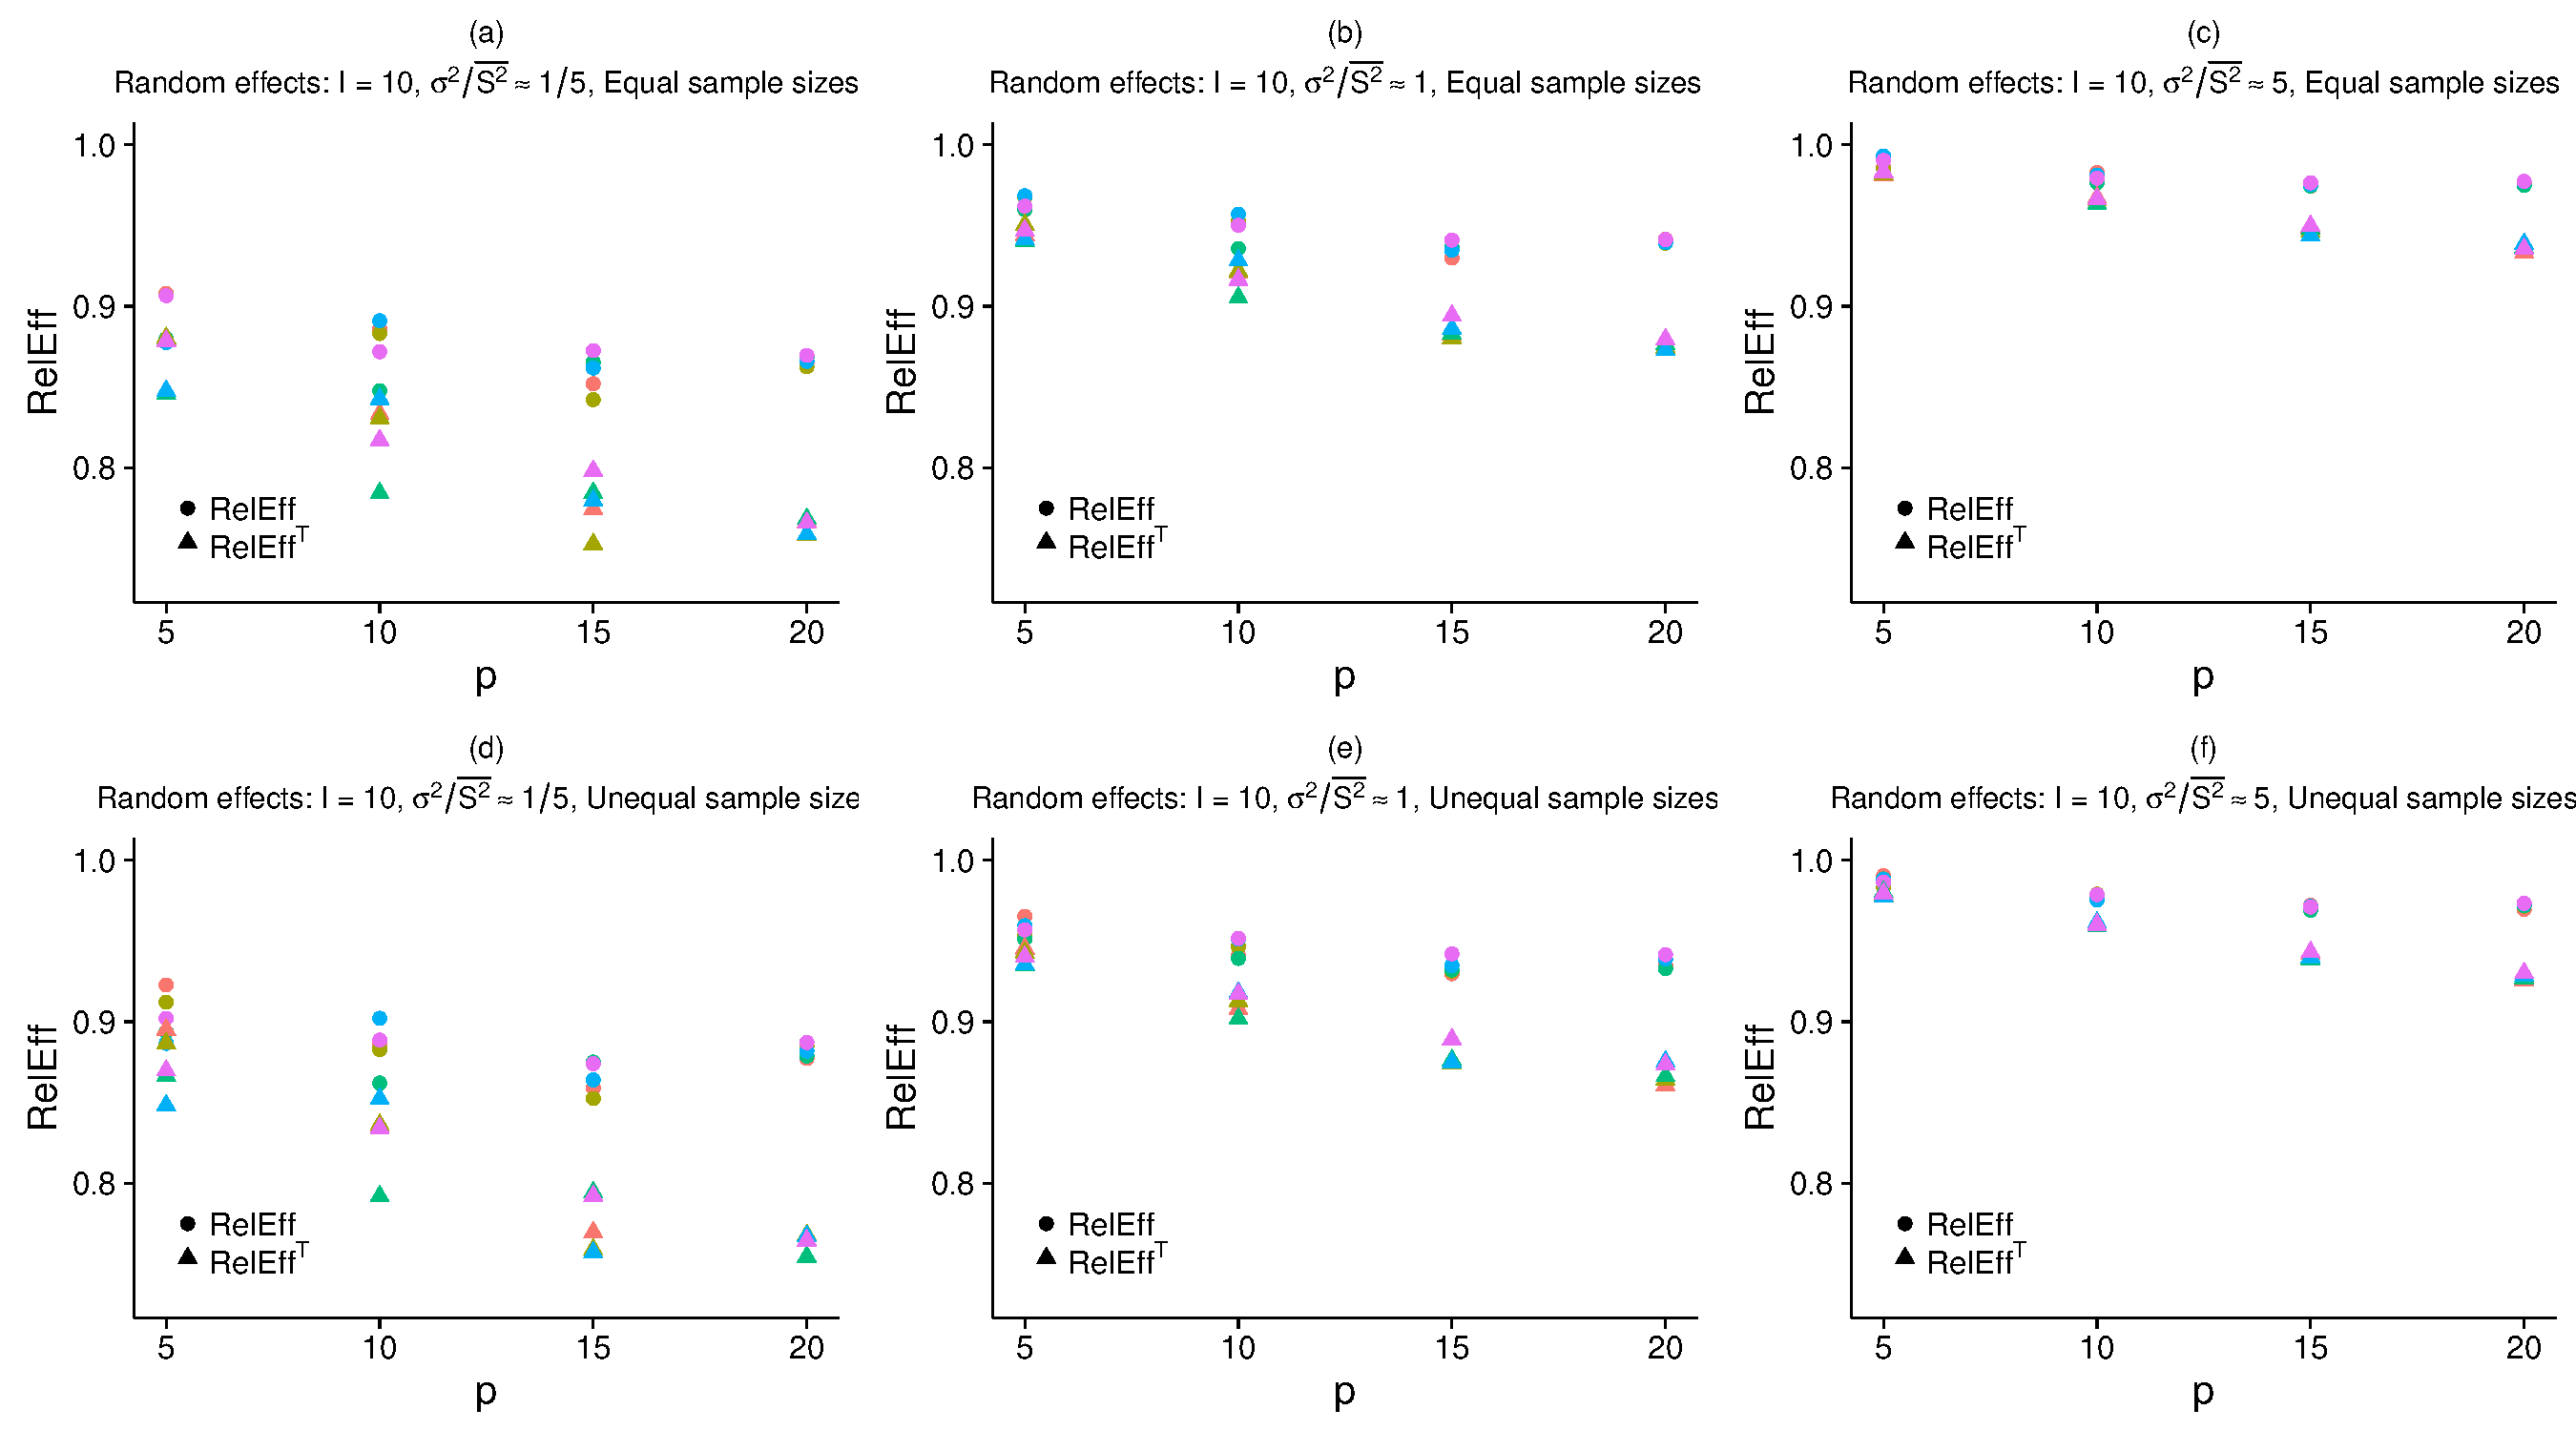
\includegraphics[width=\maxwidth]{figures/Boca_Figure_S4_panels-1} 

}



\end{knitrout}

\section{Make Figure S5}

\begin{knitrout}
\definecolor{shadecolor}{rgb}{0.969, 0.969, 0.969}\color{fgcolor}\begin{kframe}
\begin{alltt}
\hlstd{I_20_Same_Panel_A} \hlkwb{<-} \hlkwd{panelFigS4S5}\hlstd{(}\hlkwc{I}\hlstd{=}\hlnum{20}\hlstd{,} \hlkwc{subsetSigma2} \hlstd{=} \hlstr{"Sigma^2 = 1/5"}\hlstd{,} \hlkwc{RelEffSubs} \hlstd{= RelEffSame)} \hlopt{+}
  \hlkwd{labs}\hlstd{(}\hlkwc{color}\hlstd{=}\hlstr{""}\hlstd{,} \hlkwc{shape}\hlstd{=}\hlstr{""}\hlstd{,}
       \hlkwc{title}\hlstd{=}\hlkwd{expression}\hlstd{(}\hlkwd{atop}\hlstd{(}\hlstr{"(a)"}\hlstd{,} \hlkwd{paste}\hlstd{(}\hlstr{"Random effects: "}\hlstd{,}
                                          \hlstd{I,} \hlstr{" = "}\hlstd{,} \hlnum{20}\hlstd{,} \hlstr{", "}\hlstd{,}
                                          \hlstd{sigma}\hlopt{^}\hlnum{2}\hlopt{/}\hlkwd{bar}\hlstd{(S}\hlopt{^}\hlnum{2}\hlstd{),}  \hlkwd{phantom}\hlstd{()} \hlopt \hlkwd{phantom}\hlstd{() ,} \hlnum{1}\hlopt{/}\hlnum{5}\hlstd{,} \hlstr{", "}\hlstd{,}
                                          \hlstr{"Equal sample sizes"}\hlstd{))))}
\end{alltt}
\end{kframe}
\end{knitrout}

\begin{knitrout}
\definecolor{shadecolor}{rgb}{0.969, 0.969, 0.969}\color{fgcolor}\begin{kframe}
\begin{alltt}
\hlstd{I_20_Same_Panel_B} \hlkwb{<-} \hlkwd{panelFigS4S5}\hlstd{(}\hlkwc{I}\hlstd{=}\hlnum{20}\hlstd{,} \hlkwc{subsetSigma2} \hlstd{=} \hlstr{"Sigma^2 = 1"}\hlstd{,} \hlkwc{RelEffSubs} \hlstd{= RelEffSame)} \hlopt{+}
  \hlkwd{labs}\hlstd{(}\hlkwc{color}\hlstd{=}\hlstr{""}\hlstd{,} \hlkwc{shape}\hlstd{=}\hlstr{""}\hlstd{,}
       \hlkwc{title}\hlstd{=}\hlkwd{expression}\hlstd{(}\hlkwd{atop}\hlstd{(}\hlstr{"(b)"}\hlstd{,} \hlkwd{paste}\hlstd{(}\hlstr{"Random effects: "}\hlstd{,}
                                          \hlstd{I,} \hlstr{" = "}\hlstd{,} \hlnum{20}\hlstd{,} \hlstr{", "}\hlstd{,}
                                          \hlstd{sigma}\hlopt{^}\hlnum{2}\hlopt{/}\hlkwd{bar}\hlstd{(S}\hlopt{^}\hlnum{2}\hlstd{),}  \hlkwd{phantom}\hlstd{()} \hlopt \hlkwd{phantom}\hlstd{() ,} \hlnum{1}\hlstd{,} \hlstr{", "}\hlstd{,}
                                          \hlstr{"Equal sample sizes"}\hlstd{))))}
\end{alltt}
\end{kframe}
\end{knitrout}

\begin{knitrout}
\definecolor{shadecolor}{rgb}{0.969, 0.969, 0.969}\color{fgcolor}\begin{kframe}
\begin{alltt}
\hlstd{I_20_Same_Panel_C} \hlkwb{<-} \hlkwd{panelFigS4S5}\hlstd{(}\hlkwc{I}\hlstd{=}\hlnum{20}\hlstd{,} \hlkwc{subsetSigma2} \hlstd{=} \hlstr{"Sigma^2 = 5"}\hlstd{,} \hlkwc{RelEffSubs} \hlstd{= RelEffSame)} \hlopt{+}
  \hlkwd{labs}\hlstd{(}\hlkwc{color}\hlstd{=}\hlstr{""}\hlstd{,} \hlkwc{shape}\hlstd{=}\hlstr{""}\hlstd{,}
       \hlkwc{title}\hlstd{=}\hlkwd{expression}\hlstd{(}\hlkwd{atop}\hlstd{(}\hlstr{"(c)"}\hlstd{,} \hlkwd{paste}\hlstd{(}\hlstr{"Random effects: "}\hlstd{,}
                                          \hlstd{I,} \hlstr{" = "}\hlstd{,} \hlnum{20}\hlstd{,} \hlstr{", "}\hlstd{,}
                                          \hlstd{sigma}\hlopt{^}\hlnum{2}\hlopt{/}\hlkwd{bar}\hlstd{(S}\hlopt{^}\hlnum{2}\hlstd{),}  \hlkwd{phantom}\hlstd{()} \hlopt \hlkwd{phantom}\hlstd{() ,} \hlnum{5}\hlstd{,} \hlstr{", "}\hlstd{,}
                                          \hlstr{"Equal sample sizes"}\hlstd{))))}
\end{alltt}
\end{kframe}
\end{knitrout}

%%%%%%%%%%%%%%%%%%%%%%%%%%%%%%%%%%%%%%%%%%%%%%%%%%%%%%%%%%%%%%%%%%%%%%%%%%%%%%%%

\begin{knitrout}
\definecolor{shadecolor}{rgb}{0.969, 0.969, 0.969}\color{fgcolor}\begin{kframe}
\begin{alltt}
\hlstd{I_20_Diff_Panel_A} \hlkwb{<-} \hlkwd{panelFigS4S5}\hlstd{(}\hlkwc{I}\hlstd{=}\hlnum{20}\hlstd{,} \hlkwc{subsetSigma2} \hlstd{=} \hlstr{"Sigma^2 = 1/5"}\hlstd{,} \hlkwc{RelEffSubs} \hlstd{= RelEffDiff)} \hlopt{+}
  \hlkwd{labs}\hlstd{(}\hlkwc{color}\hlstd{=}\hlstr{""}\hlstd{,} \hlkwc{shape}\hlstd{=}\hlstr{""}\hlstd{,}
       \hlkwc{title}\hlstd{=}\hlkwd{expression}\hlstd{(}\hlkwd{atop}\hlstd{(}\hlstr{"(d)"}\hlstd{,} \hlkwd{paste}\hlstd{(}\hlstr{"Random effects: "}\hlstd{,}
                                          \hlstd{I,} \hlstr{" = "}\hlstd{,} \hlnum{20}\hlstd{,} \hlstr{", "}\hlstd{,}
                                          \hlstd{sigma}\hlopt{^}\hlnum{2}\hlopt{/}\hlkwd{bar}\hlstd{(S}\hlopt{^}\hlnum{2}\hlstd{),}  \hlkwd{phantom}\hlstd{()} \hlopt \hlkwd{phantom}\hlstd{() ,} \hlnum{1}\hlopt{/}\hlnum{5}\hlstd{,} \hlstr{", "}\hlstd{,}
                                          \hlstr{"Unequal sample sizes"}\hlstd{))))}
\end{alltt}
\end{kframe}
\end{knitrout}

\begin{knitrout}
\definecolor{shadecolor}{rgb}{0.969, 0.969, 0.969}\color{fgcolor}\begin{kframe}
\begin{alltt}
\hlstd{I_20_Diff_Panel_B} \hlkwb{<-} \hlkwd{panelFigS4S5}\hlstd{(}\hlkwc{I}\hlstd{=}\hlnum{20}\hlstd{,} \hlkwc{subsetSigma2} \hlstd{=} \hlstr{"Sigma^2 = 1"}\hlstd{,} \hlkwc{RelEffSubs} \hlstd{= RelEffDiff)} \hlopt{+}
  \hlkwd{labs}\hlstd{(}\hlkwc{color}\hlstd{=}\hlstr{""}\hlstd{,} \hlkwc{shape}\hlstd{=}\hlstr{""}\hlstd{,}
       \hlkwc{title}\hlstd{=}\hlkwd{expression}\hlstd{(}\hlkwd{atop}\hlstd{(}\hlstr{"(e)"}\hlstd{,} \hlkwd{paste}\hlstd{(}\hlstr{"Random effects: "}\hlstd{,}
                                          \hlstd{I,} \hlstr{" = "}\hlstd{,} \hlnum{20}\hlstd{,} \hlstr{", "}\hlstd{,}
                                          \hlstd{sigma}\hlopt{^}\hlnum{2}\hlopt{/}\hlkwd{bar}\hlstd{(S}\hlopt{^}\hlnum{2}\hlstd{),}  \hlkwd{phantom}\hlstd{()} \hlopt \hlkwd{phantom}\hlstd{() ,} \hlnum{1}\hlstd{,} \hlstr{", "}\hlstd{,}
                                          \hlstr{"Unequal sample sizes"}\hlstd{))))}
\end{alltt}
\end{kframe}
\end{knitrout}

\begin{knitrout}
\definecolor{shadecolor}{rgb}{0.969, 0.969, 0.969}\color{fgcolor}\begin{kframe}
\begin{alltt}
\hlstd{I_20_Diff_Panel_C} \hlkwb{<-} \hlkwd{panelFigS4S5}\hlstd{(}\hlkwc{I}\hlstd{=}\hlnum{20}\hlstd{,} \hlkwc{subsetSigma2} \hlstd{=} \hlstr{"Sigma^2 = 5"}\hlstd{,} \hlkwc{RelEffSubs} \hlstd{= RelEffDiff)} \hlopt{+}
  \hlkwd{labs}\hlstd{(}\hlkwc{color}\hlstd{=}\hlstr{""}\hlstd{,} \hlkwc{shape}\hlstd{=}\hlstr{""}\hlstd{,}
       \hlkwc{title}\hlstd{=}\hlkwd{expression}\hlstd{(}\hlkwd{atop}\hlstd{(}\hlstr{"(f)"}\hlstd{,} \hlkwd{paste}\hlstd{(}\hlstr{"Random effects: "}\hlstd{,}
                                          \hlstd{I,} \hlstr{" = "}\hlstd{,} \hlnum{20}\hlstd{,} \hlstr{", "}\hlstd{,}
                                          \hlstd{sigma}\hlopt{^}\hlnum{2}\hlopt{/}\hlkwd{bar}\hlstd{(S}\hlopt{^}\hlnum{2}\hlstd{),}  \hlkwd{phantom}\hlstd{()} \hlopt \hlkwd{phantom}\hlstd{() ,} \hlnum{5}\hlstd{,} \hlstr{", "}\hlstd{,}
                                          \hlstr{"Unequal sample sizes"}\hlstd{))))}
\end{alltt}
\end{kframe}
\end{knitrout}

Put all 6 panels together for Figure 5:

\begin{knitrout}
\definecolor{shadecolor}{rgb}{0.969, 0.969, 0.969}\color{fgcolor}\begin{kframe}
\begin{alltt}
\hlkwd{multiplot}\hlstd{(I_20_Same_Panel_A, I_20_Diff_Panel_A,}
          \hlstd{I_20_Same_Panel_B, I_20_Diff_Panel_B,}
          \hlstd{I_20_Same_Panel_C, I_20_Diff_Panel_C,}
          \hlkwc{cols}\hlstd{=}\hlnum{3}\hlstd{)}
\end{alltt}
\end{kframe}

{\centering 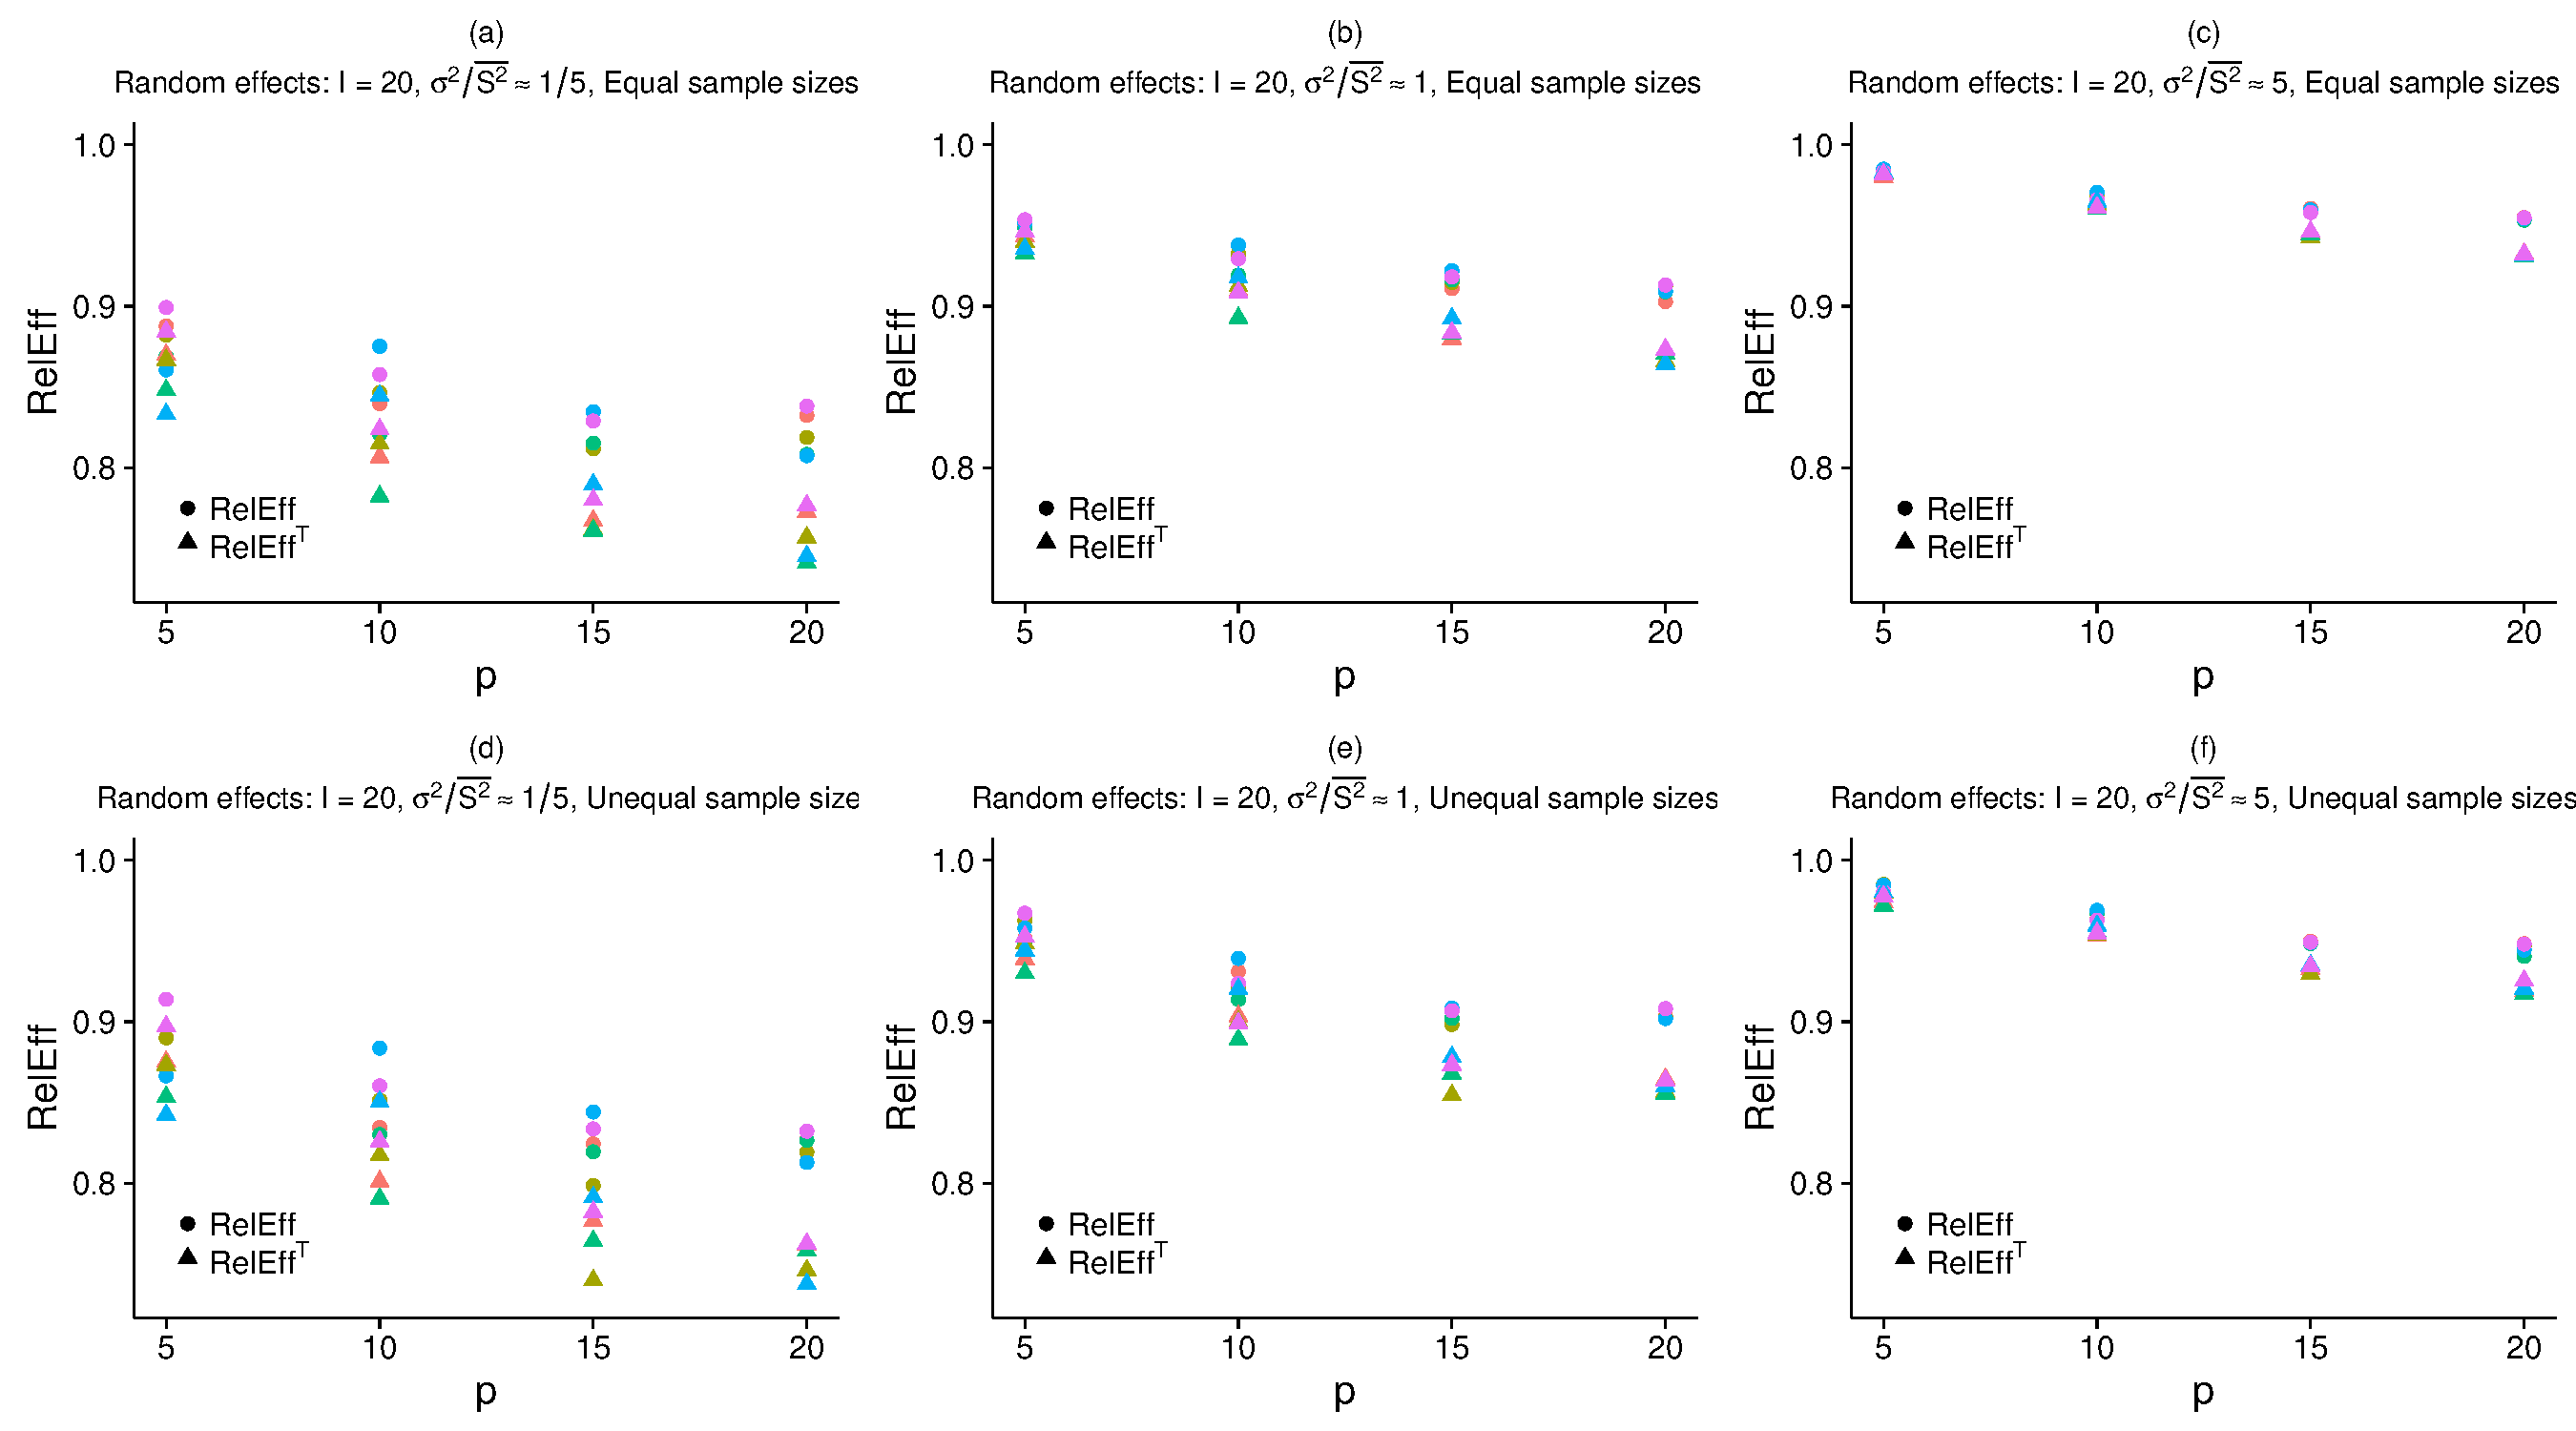
\includegraphics[width=\maxwidth]{figures/Boca_Figure_S5_panels-1} 

}



\end{knitrout}


\end{document}
